\documentclass[11pt]{article}
\usepackage{fontspec}\setmainfont{Charter}\setmonofont{Menlo}[Scale=0.82]
\usepackage{microtype}
\usepackage[a4paper,margin=27mm]{geometry}
\usepackage{booktabs,longtable,array}
\usepackage{setspace}\setstretch{1.08}
\usepackage{tikz}\usetikzlibrary{arrows.meta,positioning}\usepackage{pgfplots}\pgfplotsset{compat=1.18}
\usepackage[normalem]{ulem}
\usepackage[hidelinks]{hyperref}
\usepackage[font=small,labelfont=sc]{caption}
\usepackage{listings}
\lstset{basicstyle=\ttfamily\footnotesize,breaklines=true,columns=fullflexible,keepspaces=true,frame=leftline,framerule=0.4pt,xleftmargin=8pt,upquote=true,literate={«}{{«}}1 {»}{{»}}1 {—}{{---}}1 {–}{{--}}1 {’}{{'}}1 {“}{{``}}1 {”}{{''}}1 {é}{{\'e}}1 {è}{{\`e}}1 {à}{{\`a}}1 {ê}{{\^e}}1 {ô}{{\^o}}1 {ç}{{\c{c}}}1 {É}{{\'E}}1 {û}{{\^u}}1 {î}{{\^i}}1 {ù}{{\`u}}1}

\newcommand{\q}[1]{«\,#1\,»}
\newcommand{\qq}[1]{“#1”}
\newcommand{\lf}[3]{\href{https://grothendieck.commutator.io/\##1/#2}{#3}}
\raggedbottom\emergencystretch=1.5em
\title{\Large A Machine Reads Grothendieck's Working Notes:\\ Mathematics as TeX inside TEI, Two Registers,\\ and an Edition That Keeps None of Its Witness}
\author{Michel Hua\\ \small Commutator, Paris\\ \small \texttt{michel@commutator.io}}
\date{\small Draft of 26 September 2026, prepared for the \emph{Journal of the Text Encoding Initiative}}
\begin{document}
\maketitle

\begin{abstract}
\noindent This article reports the transcription by a large language model of the working notes of the mathematician Alexandre Grothendieck (1928--2014), held by the University of Montpellier: 178 openly accessible folders, 16,074 digitised pages, 1949 to 1991, in a hand that ran faster than it could be read and a notation of his own. The model transcribed the pages twenty at a time into a restricted LaTeX of seven apparatus macros; a mechanical converter derives from each file a TEI document in which the mathematics is carried as TeX inside \texttt{<formula>} and commutative diagrams as \texttt{tikz-cd} inside \texttt{<figure>}; a second register, a modernised reading in current notation, is derived from the transcription and never from the hand. The edition stores no page of the fonds: the facsimile beside each reading is Montpellier's own file, streamed through a relay as it is looked at. By 26 September 2026, 362 passes had read 4,955 pages in 130 folders, and the apparatus records 39,397 words left illegible, 7.2 per cent of the words read. The article sets out the encoding and its reasons, the derived registers of names, dates, letters and hands that the transcription makes possible, and the limits: nothing has been checked by a person, one macro was found carrying two senses, and TEI's formula element carries mathematics it does not describe. The use of generative AI is declared.
\end{abstract}

\noindent\textbf{Keywords.} mathematical manuscripts; large language models; transcription; critical apparatus; mathematical notation; archival rights; Alexandre Grothendieck.

\section{Introduction}

Alexandre Grothendieck left the University of Montpellier in 1991 and left his papers behind him, with his former student Jean Malgoire. They form the fonds that the university catalogued in 2015 and 2016 and has digitised in part: 178 folders in open access, 16,074 pages by the inventory's count, arranged in twenty-two groups in the order he filed them (Université de Montpellier n.d.). They are working notes. He wrote for himself, day by day, in ink and pencil, over and between his own lines; he took the same chapter up four times; he abandoned a proof and picked it up thirty pages later; he wrote on the backs of administrative letters, of seminar notes and of other people's typescripts. Some of what the folders hold has been published, much of it by mathematicians who transcribed it by hand over years --- the correspondence with Serre (Colmez and Serre 2001), \emph{À la poursuite des champs} (Maltsiniotis 2022), the texts gathered by the Grothendieck Circle (Grothendieck Circle n.d.). Most of it has not, and most of it had not been read by anyone since it was written.

This article reports an experiment in reading it with a large language model as the first transcriber, under constraints designed to make its reading checkable rather than trustworthy. It is the second report of a method first run on the ledgers of Edward and Josephine Hopper (Hua 2026), and it is written for what this corpus changes. Three things change. The document is mathematics, and mathematics is a notation before it is a language, so the question of how a transcription encodes it --- and how TEI carries it --- is the question the Hopper ledgers never raised. The corpus is two orders of magnitude larger, which turns the human check from a debt into the main fact about the edition. And the witness cannot be copied: the fonds is under copyright, a third of its pages may not be circulated at all, and the edition holds none of it, so the reading and its facsimile meet only in the reader's browser.

The objective is methodological. No claim about Grothendieck's mathematics is made here that the demonstration would need to be correct for. The article presents the fonds (Section 3), the transcription method and its rules (Section 4), the two registers (Section 5), the TEI encoding and what it does with mathematics (Section 6), the interface and the derived registers (Section 7), the findings and how they are kept from becoming claims (Section 8), and the limits (Section 9). Four words are kept apart, as in the first report: a reading is \emph{reproducible} when the process that made it can be rerun, \emph{auditable} when a reader can find the evidence for each sentence, \emph{reliable} when like cases are treated alike, and \emph{valid} when it is right. This edition claims the first three and not the fourth.

\section{Related work}

The transcription of handwriting by large language models is recent and moving. Humphries and colleagues (2025) report character error rates of about six to seven per cent for general-purpose models on eighteenth- and nineteenth-century English manuscripts; Crosilla, Klic and Colavizza (2025) benchmark several models and discuss when a model's linguistic prior helps and when it hinders. Mathematics is the extreme case of the second. A model that has read a great deal of mathematics will complete a formula as readily as it completes a sentence, and a completed formula is the more dangerous of the two, because it is well-formed: an index that makes an identity true is not a reading of the index on the page. The rule this edition sets against that prior --- nothing illegible is guessed, even where the mathematics would supply it --- is the one that shapes everything else, and Section 9 measures what it costs.

The evaluation of models as producers of TEI is more recent still. Strutz (2026) proposes a framework for assessing model-generated TEI from syntactic validity to semantic accuracy. As in the first report, the model here writes no TEI at all: it writes a restricted language whose macros correspond one to one with TEI constructs, and the TEI is derived. The precedent for a reduced intermediate language converted up into conformant TEI is Cummings and Willcox (2013), whose \texttt{tei\_corset} bounded what a keying company could write; these macros bound what a model may write, and the consequence is shared, that the converter must be something a test can hold to account.

Mathematics in TEI has a short answer in the Guidelines and a long one outside them. The Guidelines provide \texttt{<formula>}, whose \texttt{@notation} names the notation the content is in, and leave that content to another vocabulary: MathML, TeX, or an image (TEI Consortium 2026). MathML is the W3C's vocabulary for mathematical structure and presentation (W3C 2014), and a TEI file may embed it. Section 6 explains why this edition carries TeX instead, and what that choice gives up. Hand attribution, which the first report treated at length, is a lesser question here: the fonds is in one hand, his, except where it holds other people's letters and typescripts, and those are marked by what they are rather than by their letterforms (Stokes 2015).

\section{The fonds}

\subsection{The inventory, and the three numberings}

The inventory of the fonds is complete and rigorous, and was made for an archive and not for a reader. Each folder has a shelfmark (\texttt{19}, \texttt{140-2}, \texttt{156-9}), a title --- his, pencilled on the cover, or the archivists', in square brackets where the folder bore none --- a dating, and a page count; the folders stand in twenty-two groups, from \emph{Cristaux} and \emph{Théorie des motifs} to the \emph{Longue marche à travers la théorie de Galois} and \emph{Dérivateurs}. Each folder is served as one PDF, between 4 and 270 megabytes.

Three numberings overlap on every page. Grothendieck's own, where he paginated: the Long March runs from 1 to 787 across four boxes. The archivists', pencilled at the foot of every page, which is what the inventory counts and what the edition calls a page. And the PDF's, one ahead of the archivists', because the university's file opens on a generated cover. The edition addresses a page by the archivists' number and converts to the PDF's only at the last moment, when it asks Montpellier for a page; a reading that cited the PDF's number would cite a sheet the archivists never numbered.

\subsection{What the pages are}

The pages are drafts, and the drafting is the object. A restart is not a repetition to delete. A verso is often unrelated to its recto --- an administrative letter, a typescript returned by a secretary --- and was digitised deliberately, sometimes upside down. The dates are nearly all inferred. Figure~\ref{fig:dating} sets the inventory's datings against the dates the transcriptions have found written on the leaves: of the 153 folders the inventory dates, 111 rest in part on a deduction the archivists mark with their square brackets, and 25 more are \q{s.d.}, undated; the transcriptions have found 160 dates on the leaves themselves, in 52 folders, 47 of them machine stamps on the computer listings whose backs he wrote on in the 1980s, which date the paper and not the writing.

\begin{figure}[htbp]\centering
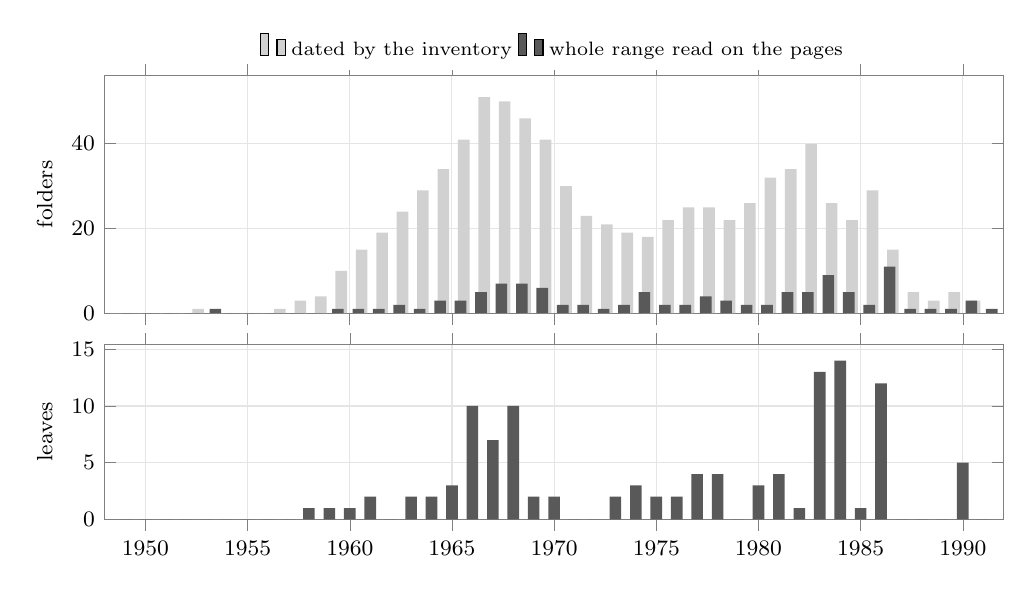
\begin{tikzpicture}
\begin{axis}[name=top,width=13cm,height=4.6cm,xmin=1948,xmax=1992,ymin=0,
  xticklabels={},ylabel={folders},ybar,bar width=4.2pt,grid=major,grid style={black!10},
  tick label style={font=\footnotesize},label style={font=\footnotesize},axis line style={black!50},
  legend style={font=\scriptsize,draw=none,at={(0.5,1.02)},anchor=south},legend columns=2,legend cell align=left]
\addplot[fill=black!18,draw=none] coordinates {(1949,0) (1950,0) (1951,0) (1952,0) (1953,1) (1954,0) (1955,0) (1956,0) (1957,1) (1958,3) (1959,4) (1960,10) (1961,15) (1962,19) (1963,24) (1964,29) (1965,34) (1966,41) (1967,51) (1968,50) (1969,46) (1970,41) (1971,30) (1972,23) (1973,21) (1974,19) (1975,18) (1976,22) (1977,25) (1978,25) (1979,22) (1980,26) (1981,32) (1982,34) (1983,40) (1984,26) (1985,22) (1986,29) (1987,15) (1988,5) (1989,3) (1990,5) (1991,3)};
\addplot[fill=black!65,draw=none] coordinates {(1949,0) (1950,0) (1951,0) (1952,0) (1953,1) (1954,0) (1955,0) (1956,0) (1957,0) (1958,0) (1959,1) (1960,1) (1961,1) (1962,2) (1963,1) (1964,3) (1965,3) (1966,5) (1967,7) (1968,7) (1969,6) (1970,2) (1971,2) (1972,1) (1973,2) (1974,5) (1975,2) (1976,2) (1977,4) (1978,3) (1979,2) (1980,2) (1981,5) (1982,5) (1983,9) (1984,5) (1985,2) (1986,11) (1987,1) (1988,1) (1989,1) (1990,3) (1991,1)};
\legend{dated by the inventory, whole range read on the pages}
\end{axis}
\begin{axis}[at={(top.south)},anchor=north,yshift=-4mm,width=13cm,height=3.8cm,xmin=1948,xmax=1992,ymin=0,
  ylabel={leaves},ybar,bar width=4.2pt,grid=major,grid style={black!10},xtick={1950,1955,1960,1965,1970,1975,1980,1985,1990},
  x tick label style={/pgf/number format/1000 sep={}},
  tick label style={font=\footnotesize},label style={font=\footnotesize},axis line style={black!50}]
\addplot[fill=black!65,draw=none] coordinates {(1949,0) (1950,0) (1951,0) (1952,0) (1953,0) (1954,0) (1955,0) (1956,0) (1957,0) (1958,1) (1959,1) (1960,1) (1961,2) (1962,0) (1963,2) (1964,2) (1965,3) (1966,10) (1967,7) (1968,10) (1969,2) (1970,2) (1971,0) (1972,0) (1973,2) (1974,3) (1975,2) (1976,2) (1977,4) (1978,4) (1979,0) (1980,3) (1981,4) (1982,1) (1983,13) (1984,14) (1985,1) (1986,12) (1987,0) (1988,0) (1989,0) (1990,5) (1991,0)};
\end{axis}
\end{tikzpicture}
\caption{Two kinds of date on one axis, each on its own scale. Above: for each year, how many of the 153 dated folders the inventory's ranges cover (an open end, « à partir de 1982 », counted five years on), and, darker, how many of them rest on a range the archivists read on the pages rather than deduced in their square brackets; 25 folders are « s.d. ». Below: the 113 dates the transcriptions have found written on the leaves themselves, machine stamps on reused paper left out. From \texttt{src/content/catalogue.ts} and \texttt{src/content/dated-leaves.json} (2026-09-26), after the site's page \emph{Timeline}.}\label{fig:dating}
\end{figure}


\subsection{What may be read, and what was}

Of the fonds' some 28,000 pages, about 18,000 may be circulated; third-party correspondence may not, without permission. The 178 folders in open access hold 16,074 pages, which at twenty pages to a batch make 884 batches. Twenty folders --- 5,129 pages, 266 batches --- are already edited by mathematicians, among them the \emph{Dérivateurs}, the Long March, \emph{Pursuing Stacks} and the \emph{Esquisse d'un programme}, and the edition marks them and links to the edition rather than read them again, since a machine's first pass beside a scholar's edition is waste. Table~\ref{tab:coverage} gives the state of the reading on 26 September 2026.

\begin{table}[htbp]\centering\small
\caption{The fonds as counted on 26 September 2026: the inventory, the part already edited by others and set aside, and what the passes have read. A batch is twenty of the archivists' pages; a transcribed page is one that carries mathematics, the others being skipped by rule.}\label{tab:coverage}
\begin{tabular}{lrrr}\toprule
 & Folders & Pages & Batches\\\midrule
Open access (inventory) & 178 & 16,074 & 884\\
Already edited, set aside & 20 & 5,129 & 266\\
Left to this edition & 158 & 10,945 & 618\\\midrule
Begun & 130 & & \\
Transcribed & & 4,955 & 362\\
Read whole and modernised & 72 & & 187\\\bottomrule
\end{tabular}
\end{table}

\section{The transcription method}

% The schema this edition shares with the Hopper edition, and its values here.
%
% Drawn rather than generated, because it states decisions and not data. The
% upper row is the schema: five stations and one loop. The lower row, in grey,
% is the same schema with this edition's values filled in.
\begin{figure}[htbp]\centering
\resizebox{0.96\textwidth}{!}{%
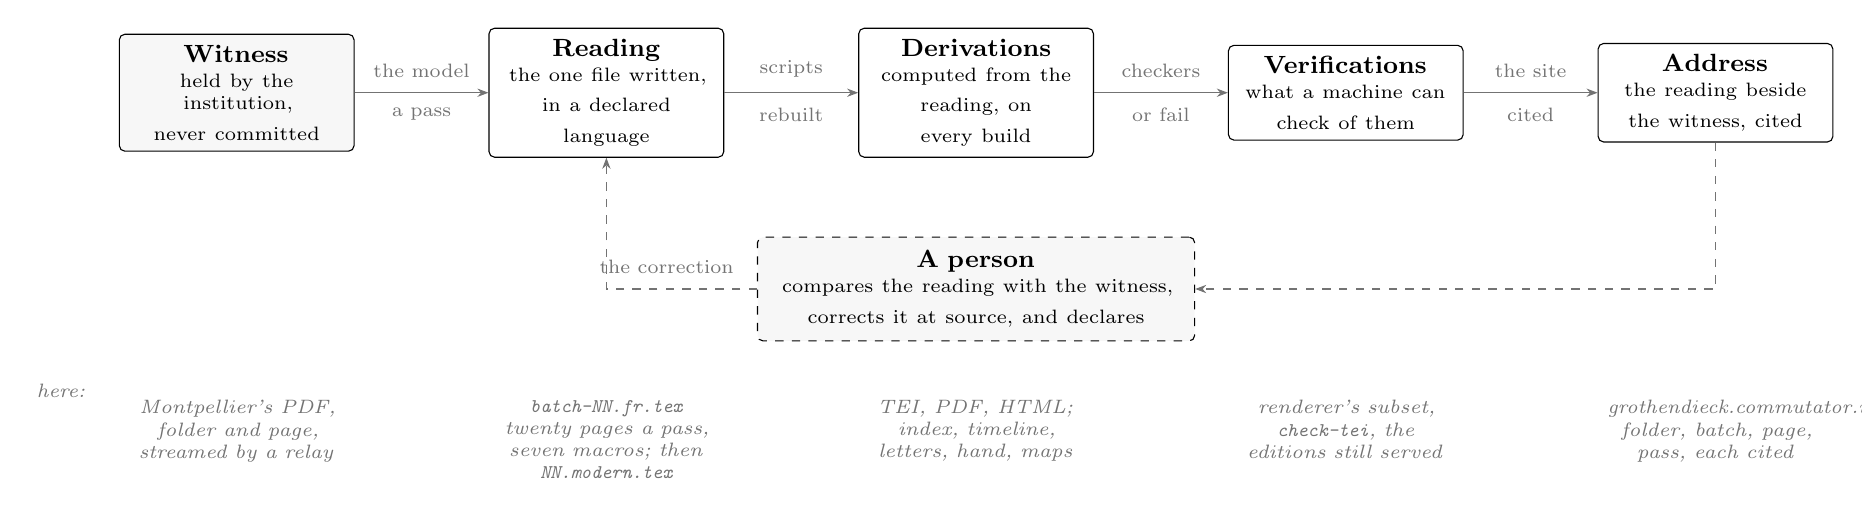
\begin{tikzpicture}[
  font=\small,
  st/.style={draw, rounded corners=2pt, align=center, inner sep=4pt,
             minimum height=12mm, text width=27mm},
  src/.style={st, fill=black!3},
  inst/.style={font=\scriptsize\itshape, text=black!55, align=center,
               text width=27mm, anchor=north},
  lbl/.style={font=\scriptsize, text=black!55, align=center},
  arr/.style={-{Stealth[length=4pt]}, draw=black!55},
  human/.style={arr, dashed},
]

% The schema: five stations.
\node[src] (W) {\textbf{Witness}\\[1pt]\scriptsize held by the institution,\\\scriptsize never committed};
\node[st, right=17mm of W] (R) {\textbf{Reading}\\[1pt]\scriptsize the one file written,\\\scriptsize in a declared language};
\node[st, right=17mm of R] (D) {\textbf{Derivations}\\[1pt]\scriptsize computed from the\\\scriptsize reading, on every build};
\node[st, right=17mm of D] (V) {\textbf{Verifications}\\[1pt]\scriptsize what a machine can\\\scriptsize check of them};
\node[st, right=17mm of V] (A) {\textbf{Address}\\[1pt]\scriptsize the reading beside\\\scriptsize the witness, cited};

\draw[arr] (W) -- node[lbl, above=2pt]{the model} node[lbl, below=2pt]{a pass} (R);
\draw[arr] (R) -- node[lbl, above=2pt]{scripts} node[lbl, below=2pt]{rebuilt} (D);
\draw[arr] (D) -- node[lbl, above=2pt]{checkers} node[lbl, below=2pt]{or fail} (V);
\draw[arr] (V) -- node[lbl, above=2pt]{the site} node[lbl, below=2pt]{cited} (A);

% The loop: the only step no file can prove, and the only one that changes the reading.
\node[st, dashed, fill=black!3, below=10mm of D, text width=52mm, inner sep=5pt] (P)
  {\textbf{A person}\\[1pt]\scriptsize compares the reading with the witness,\\\scriptsize corrects it at source, and declares};
\draw[human] (A.south) |- (P.east);
\draw[human] (P.west) -| node[lbl, above=2pt, pos=0.3]{the correction} (R.south);

% The same schema, with this edition's values.
\node[inst, below=5mm of P.south, text width=0mm] (anchor) {};
\node[inst] at (W |- anchor) {Montpellier's PDF,\\folder and page,\\streamed by a relay};
\node[inst] at (R |- anchor) {\texttt{batch-NN.fr.tex}\\twenty pages a pass,\\seven macros; then\\\texttt{NN.modern.tex}};
\node[inst] at (D |- anchor) {TEI, PDF, HTML;\\index, timeline,\\letters, hand, maps};
\node[inst] at (V |- anchor) {renderer's subset,\\\texttt{check-tei}, the\\editions still served};
\node[inst] at (A |- anchor) {grothendieck.commutator.io\\folder, batch, page,\\pass, each cited};
\node[lbl, anchor=east, xshift=-3mm] at (W.west |- anchor) {\itshape here:};

\end{tikzpicture}}
\caption{The schema this edition shares with its sibling on the Hopper ledgers
(Hua 2026), and its values in this one. Five stations and one loop: the model turns a witness into a reading, in
passes whose header names the model and the date; scripts derive everything
else from the reading and regenerate it on every build; checkers fail the build
on what a machine can check; the site places the reading beside the witness
and cites both by reference. The dashed loop is the person, who compares the
reading with the witness and corrects the reading, which alone changes anything
downstream. Four invariants hold at every station: the witness is never committed;
only the reading is written, everything else is derived and compared; every
assertion carries an address into the witness; and the person's verdict is
declared, not observed. The grey row gives this edition's values. Figure by the
author.}\label{fig:pipeline}
\end{figure}


\subsection{The schema, and its values here}

Figure~\ref{fig:pipeline} gives the arrangement, which is the one the first report describes and which this edition was in fact the first to run: a \emph{witness} held by the institution and never committed; a \emph{reading}, the one file that is written, by the model first and by a person thereafter, in a language whose every construct is declared; \emph{derivations}, computed from the reading by scripts on every build; \emph{verifications}, whatever a machine can check of them; and an \emph{address}, the reading placed beside its witness and cited by the holder's reference and the edition's dated pass. The loop is the person. What distinguishes this edition from the ledgers' is only the values the stations take, and three of them are new: a model that reads and then restates, a witness that cannot be mirrored for the reader, and a notation that is not text.

\subsection{The unit of work and the model}

A batch is twenty of the archivists' pages, read in one fresh model context and written as a single file, \texttt{transcripts/<folder>/batch-NN.fr.tex}. The ceiling is not arbitrary. Past twenty pages of this hand, the reading degrades towards the end of the pass with nothing in the output to signal it, and a transcription whose weakening point is unknown cannot be used. The skill that performs the reading admits named models and refuses any other, and each file's header records the model and the date in a fixed form, \texttt{\% Pass: Opus 5.5 (claude-opus-5-5), <date> --- first pass, unchecked against the pages by a human}, so that provenance is a fact about the file and not about the session. Of the 362 first passes, 229 were read by Claude Opus 5.5, 102 by Claude Opus 5, 26 by Claude Fable 5.1 and 5 by Claude Fable 5; the Fable models were withdrawn for new passes on 22 September 2026, and the files they read stay as they are, their headers saying so. Twenty-seven files in fifteen folders carry a later machine revision below the first pass, dated and attributed in the same way, and none of these is a human check. The batches of a folder may run in parallel, one model context each; the price is continuity, since no batch can read the one before it, and each header says where a run crosses its boundary.

Two aids are handed to every pass, and neither is allowed to settle a reading. The first is a set of tiles: each page cut into six overlapping crops at 700 dpi, with the margin turned upright, because choosing crop rectangles by hand cost one early batch some ninety commands for sixteen pages, and choosing rectangles is not reading. The second is a lexicon of his vocabulary, abbreviations and notation, counted over every transcription so far and regenerated after each run, which keeps apart the words read plainly, the words read with doubt, and the words that occur only in doubt. A pass reading a hard leaf is rarely choosing between a word and no word; it is choosing between candidates, and the candidate that belongs to this material is the one the lexicon shows. It is built from unverified transcriptions without circularity, because it makes no claim about ink: that \emph{principal} is common in these pages is settled by hundreds of plain occurrences, and whether one stroke reads \emph{principaux} is left to the page.

\subsection{The rules}

The governing rule is the ledgers' rule translated: an invented word in a letter is a bad reading; an invented index in a formula is a theorem nobody proved. Nothing illegible is guessed, and the mark for an illegible word is never replaced by what the mathematics would require. A reading offered with doubt is marked doubtful. His language stays his --- his spelling, his punctuation, his long sentences, his slips, flagged and not corrected --- and so does the transcriber's, since every note is in French, so that the edition a French reader reads straight through has no seam in it.

The transcription is not diplomatic, and says so. The archive's material apparatus --- which verso carried which letter, where a separator sheet fell, which page was scanned upside down --- is not its subject; a page that carries no mathematics is simply absent, and the gap in the page numbers is the record. Where a page is too crowded to render whole, the mathematics is transcribed and the surrounding prose compressed, with a note. Commutative diagrams go into \texttt{tikz-cd}, never into prose, because that is the notation the mathematics of this fonds is now read in. His own prose stays whenever it is about the mathematics, and it often is: where he stops to say why a definition is the right one, that is the content. What he struck out stays, marked, because a deletion shows where the thought turned.

Three rules concern other people. A typescript or a mémoire by someone else is given as a note per page and his marks on it in full, not transcribed; a letter to him is transcribed in full where its writer is a public figure and is otherwise summarised, its writer unnamed; and letters already published in the correspondence with Serre stay condensed to their statements and a summary. Each rule answers a right that the edition does not hold.

\subsection{What the model writes}

The model writes a restricted LaTeX. Its apparatus is seven macros (Table~\ref{tab:macros}); the mathematics is ordinary LaTeX mathematics, inline and displayed, with the environments a working mathematician uses and \texttt{tikz-cd} for diagrams. Six declarations open each file --- the shelfmark, the batch, its pages, the inventory's dating copied verbatim with its brackets, the folder's title, and a watermark reading \emph{Édition de démonstration} that the PDF prints across every page, because a file without it would claim by silence a status it does not have.

\begin{table}[htbp]\centering\small
\caption{The apparatus macros, as the transcription skill declares them, and the TEI elements the converter maps them to. The mathematics itself is carried as TeX (Section 6).}\label{tab:macros}
\begin{tabular}{lp{5.3cm}l}\toprule
Macro & Meaning & TEI\\\midrule
\texttt{\textbackslash page\{47\}} & Page 47 begins, in the archivists' numbering & \texttt{pb} with \texttt{@n}, \texttt{@facs}\\
\texttt{\textbackslash ill\{\}} & Illegible; never guessed & \texttt{gap reason="illegible"}\\
\texttt{\textbackslash uncertain\{…\}} & A reading offered and flagged & \texttt{unclear}\\
\texttt{\textbackslash add\{…\}} & An editorial addition: a missing letter, an implied word & \texttt{supplied resp="\#pass"}\\
\texttt{\textbackslash struck\{…\}} & Struck out by Grothendieck & \texttt{del}\\
\texttt{\textbackslash note\{…\}} & The transcriber's note, about the mathematics & \texttt{note type="editorial"}\\
\texttt{\textbackslash marginal\{…\}} & A marginal note of his & \texttt{note type="authorial" place="margin"}\\\bottomrule
\end{tabular}
\end{table}

The subset is policed by the renderer that turns each file into the site's reading view, and the policing is weaker than it should be, which is worth saying exactly. An unknown environment is refused, naming the file and the line, and an unknown inline macro is reported rather than flattened; but a refusal is a warning, the script still exits cleanly, and the build that deploys the site goes on. Three further failures pass the renderer silently and are recorded in the repository as such because they were found late: a backslash-newline inside inline mathematics, a page-range declaration without a blank line before it, and presentational macros such as \texttt{\textbackslash underline} in running prose, which the renderer prints as text. A second check, run over the TEI on request, counts control sequences left as text; it found some thirty files carrying them in September 2026, which were corrected at source, and its last run was clean. Neither check yet fails the build, and making them do so is the cheapest improvement the edition could make.

\subsection{A transcribed page}

The following is page 8 of folder 19, \emph{Topos}, from the first batch the edition transcribed of it, as the converter exports it (the page is \lf{19}{1}{folder 19, batch 1}). The mathematics is TeX inside \texttt{<formula>}; the diagram is a figure; the note is the transcriber's and the marginal his; the struck \(\varphi\) and what replaced it are both kept.

\begin{lstlisting}
<pb n="8" facs="https://grothendieck.umontpellier.fr/19.pdf#page=9"/>
<p>qui s'expliciteront en termes des <formula notation="TeX">\varphi_{ji} = f_{j} g_{i}</formula>, [...]
<formula notation="TeX" rend="display">\lambda_{kji} : \varphi_{ki} \longrightarrow
  \varphi_{kj} \circ \varphi_{ji} \tag{3.10}</formula></p>
<p><figure type="diagram"><formula notation="tikz-cd">\begin{tikzcd}[column sep=small, row sep=small]
\varphi_{ki} \arrow[r, "\lambda_{kji}"] \arrow[d, no head] & \varphi_{kj}\varphi_{ji} \arrow[d, no head] \\
f_{k} g_{i} & f_{k}\, g_{j} f_{j}\, g_{i}
\end{tikzcd}</formula></figure></p>
<p><note type="editorial" resp="#pass">la flèche provient du morphisme d'adjonction
<formula notation="TeX">\mathrm{id} \to g_{j} f_{j}</formula>, que l'auteur indique par une
flèche verticale sous <formula notation="TeX">g_{j} f_{j}</formula></note></p>
<p><note type="authorial" place="margin">pour <formula notation="TeX">i = j = k</formula>,
<formula notation="TeX">\lambda_{kji}</formula> n'est autre que
<formula notation="TeX">\lambda_{i}</formula></note></p>
<p>[Le cas le plus intéressant est celui où les <del><formula notation="TeX">\varphi</formula></del>
<supplied resp="#pass"><formula notation="TeX">\alpha_{i}</formula></supplied> sont des
isomorphismes (i.e. les <formula notation="TeX">g_{i}</formula> pleinement fidèles). [...]</p>
\end{lstlisting}

The last paragraph shows the limit Section 9.2 takes up. The \(\alpha_i\) is his, written over the \(\varphi\) he struck; the converter, following the macro's declared sense, credits it to the transcriber.

\section{Two registers}

The ledgers of the first report needed one text. This fonds needs two, and the reason is the notation. A price of 1927 means what it meant; a \(\mathcal{C}\) of 1962 is not drawn like one of 1986, a sheaf of the Séminaire is not named as a sheaf is named today, and a reader who meets \q{fppf} spelled out on one page and reduced to initials on the next needs to be told it is the same topology. So every folder read whole yields a second document, the \emph{modernised reading}: a résumé written for someone who has not met the subject, then the mathematics in current notation and current names, with footnotes carrying everything the transcription's apparatus carried.

Three decisions govern it. The modernised reading is derived from the transcription and never from the hand: two independent readings of one hand would diverge, and nothing would say which was right. It is made per folder and not per batch, because its job is to make an argument run continuously and his arguments do not stop where the batches do. And it is the one document allowed to depart from the page, which is why it is held to a different standard from the transcription: not \emph{faithful} but \emph{correct as it stands}. Where the manuscript is loose, the reading states what is true and footnotes what the page has. The standard is a reasoning standard, calibrated against one reference reading and stated in the skill as four failure modes to check: a statement strengthened beyond what the page proves, a hypothesis dropped, a notation modernised into a different object, and a gap closed silently.

The résumé closes on a line of English keywords, the modern vocabulary to search under. They are the one piece of either register that is written for search rather than for reading, and the edition treats them as such: they are what the site's search, its index of subjects and its map of the mathematics are built from (Section 7.3), and they are said to be the reading's and not the page's. On 26 September 2026 seventy-two folders had been read whole in this way, carrying 1,447 keywords.

\section{The TEI encoding}

\subsection{Derived, not written}

Every transcription is exported to TEI P5 by a script that reads the \texttt{.tex} and nothing else --- not the facsimile, not the rendered HTML. The mapping is the one of Table~\ref{tab:macros} and no richer. The reasons are those of the first report: a model asked for TEI writes it fluently, and fluency is the hazard, since well-formed markup with an invented attribute has no structural signature; a seven-macro language has a small surface and each macro answers one editorial question; and because the TEI is derived, a difference between a file and its TEI is a bug in the converter and not a judgement. The LaTeX with seven private macros is legible only to this repository. TEI is what an archive, a deposit or another editor can take in without the edition's rendering chain, and a transcription that can be cited only through this site dies with it.

The header carries what the file's comment carries, in a form a machine can read. The responsibility statement names the model as a \texttt{<name type="model">} with an identifier every editorial note points to, and dates the pass; the edition statement repeats the watermark; the availability is \texttt{restricted} and says why --- the fonds is under copyright, the transcription is an unauthorised demonstration, no image is reproduced; the manuscript description carries the shelfmark, the folder's title as the inventory gives it, and the inventory's dating in an \texttt{<origDate>} with a note that the brackets are the archivists'; and the surrogate is Montpellier's PDF, with a note explaining that each page break's \texttt{@facs} points one page ahead of its \texttt{@n}, because of the generated cover.

\subsection{Mathematics as TeX}

Mathematics is carried as TeX, untouched, inside \texttt{<formula notation="TeX">}, displayed formulas marked with \texttt{@rend}, and a commutative diagram as \texttt{<figure type="diagram">} holding a \texttt{<formula notation="tikz-cd">}. TEI does not try to encode the mathematics, and neither does the converter. There are three reasons, and one cost.

The first is that the transcription is TeX already, and TeX is closer to what he wrote than MathML would be. He wrote a notation, not a structure: an underlined \(\omega\), a doubly underlined \(\Sigma\), a tilde that distinguishes two coverings, a letter he used for two objects on one page. A presentation MathML of these would be a second transcription of the first, and a content MathML would be an interpretation --- which is the modernised reading's work, and belongs in that register. The second is the apparatus. An illegible exponent or a doubtful index is an apparatus mark inside a formula, and the transcription writes it there, as \texttt{\textbackslash ill\{\}} inside \texttt{\$…\$}; kept as TeX, it stays where both the browser's renderer (KaTeX) and the PDF read it. A conversion to MathML would have to decide what an illegible subscript is, structurally, and there is no honest answer. The third is the round trip: the TeX inside the TEI is the TeX of the source, character for character, so the TEI can be checked against the \texttt{.tex} by comparing strings.

The cost is that the TEI says nothing about the mathematics that a TEI processor can use. A reader of the TEI can find every formula and cannot search inside one; the 1,330 commutative diagrams are figures whose content is opaque to the schema. And an apparatus mark inside a formula is invisible to TEI: a count of \texttt{<gap>} elements over the corpus misses every illegible index, which is why the edition's own counts (Section 7.3) are taken from the source and not from the TEI. The choice is recorded as a choice. MathML can be derived later from the same TeX, where the TeX is clean enough to support it, without touching the transcription. This article, encoded against the journal's own customisation, meets the question from the other side: that customisation admits no \texttt{<formula>}, and the article's TEI carries its few inline symbols as Unicode.

\subsection{Validation, and what is not yet validated}

Each TEI file is checked for well-formedness as it is written, where the checker is installed, and a second script reads the TEI's text for leaked control sequences, the silent failure of Section 4.4. Validation against \texttt{tei\_all} is a separate step, run by hand because the schema is a megabyte nobody wants vendored; it was last run on 5 September 2026, over the 53 files that then existed, and is not part of the build. The edition has, as yet, no customisation of its own. Its sibling on the Hopper ledgers learned the cost of that the hard way --- a corpus of well-formed files that were all invalid, because nothing had asked --- and wrote an ODD declaring exactly the elements its converter emits (Hua 2026). This edition's converter emits sixty-two element types across the corpus, header included, and would take an ODD of that size; until it has one, and until validation runs on every build, a deposit of its TEI is, in the first report's phrase, a deposit of XML.

A second debt is in the header. The export records the first pass and no other: the twenty-seven files that carry a later machine revision lose it in the TEI, which therefore names one model and one date for a file two passes produced. The \texttt{<revisionDesc>} the converter already writes is where those passes belong. Both debts are stated here as the principal encoding work the edition owes.

\section{Interface and reproducibility}

\subsection{A facsimile the edition does not hold}

The site at \url{https://grothendieck.commutator.io} renders the transcription in one pane and Montpellier's facsimile in the other, and scrolling the transcription past a page break turns the facsimile to that page. The edition holds no page of the fonds: not in the repository, whose ignore file refuses PDF outright, and not on the server. The facsimile is Montpellier's own file.

Pointing an embedded frame at Montpellier's server does not work, for three reasons measured and recorded in the repository: the server sends \texttt{X-Frame-Options: SAMEORIGIN}, which forbids any other site from framing its files; its certificate had expired on 10 December 2025, so a framed load fails verification and the warning cannot render inside a frame; and it sends no cross-origin headers, so a script cannot fetch the file either. All three are enforced by the browser against the remote origin, and none applies to a request made by a server. So a relay on the edition's origin requests the file and passes the bytes through, verified byte-identical, forwarding range requests: opening page 221 of the 204-megabyte second volume of the Long March moves 256 kilobytes in a fifth of a second. The relay is a small Node service because skipping verification of an expired certificate needs an option that no edge runtime offers; it serves only an allowlist of the folders' own files, which the build checks against the inventory; and it stores nothing.

This arrangement is an editorial fact and not only a technical one. The reading can be checked against its witness only while the witness answers. When Montpellier is down, the pane says so rather than offering a copy, and a rule of the repository forbids serving the local mirror the transcription passes read from, even in development. A reading beside an image the edition holds is a reading beside a copy; a reading beside the institution's own file is a reading beside the witness, and the difference is what a citation of it means.

\subsection{Observed, not declared}

Everything the site shows beyond the transcription is derived from it, and the counts of what exists are observed from the files and never kept by hand. The manifest of what is transcribed is built from the files present; a batch counts as transcribed once its LaTeX exists and as modernised once the folder's reading does, and neither claims that anyone has checked it. The site's progress figure is computed against the folders nobody has edited, and prints beside it the figure against the whole fonds, because narrowing a denominator flatters a ratio for free.

\subsection{Registers derived from the reading}

Once the transcription is a constrained language rather than a document, a question put to the fonds becomes a script. The edition publishes five such registers, each regenerated from the files and each resting, entry by entry, on a file and a line.

\emph{The hand} counts the apparatus per batch and per folder: of 505,862 words read by 26 September 2026, 39,397 were left illegible, 7.2 per cent; 26,428 readings were marked doubtful; he struck 20,633 times and the transcriptions record 6,144 insertions and 3,230 marginal notes; there are 1,330 commutative diagrams and 156 drawings described in notes. Figure~\ref{fig:hand} places each folder's share of unread words against its inventory dating. The figure is a count of the apparatus and not of the ink, and says so in its caption: an \texttt{\textbackslash ill\{\}} is a word one pass could not read, a fact about the hand and the pass at once.

\begin{figure}[htbp]\centering
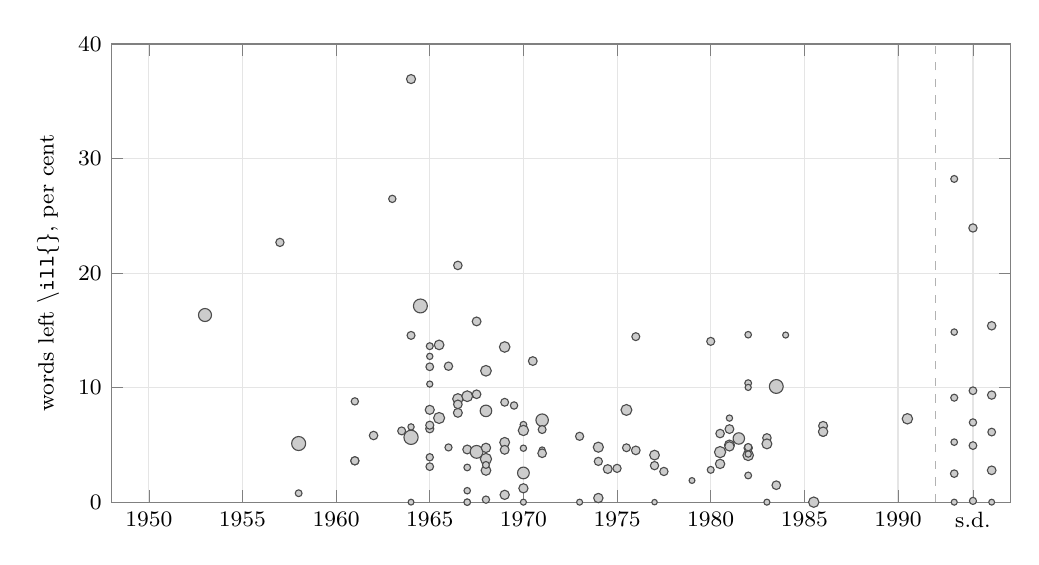
\begin{tikzpicture}
\begin{axis}[width=13cm,height=7.4cm,xmin=1948,xmax=1996,ymin=0,ymax=40,
  xtick={1950,1955,1960,1965,1970,1975,1980,1985,1990,1994},xticklabels={1950,1955,1960,1965,1970,1975,1980,1985,1990,s.d.},
  ylabel={words left \texttt{\textbackslash ill\{\}}, per cent},grid=major,grid style={black!10},
  tick label style={font=\footnotesize},label style={font=\footnotesize},axis line style={black!50}]
\draw[black!30,dashed] (axis cs:1992,0) -- (axis cs:1992,40);
\addplot[scatter,only marks,mark=*,scatter/use mapped color={draw=black!70,fill=black!20},
  visualization depends on={\thisrow{p} \as \p},scatter/@pre marker code/.append style={/tikz/mark size={0.8pt+0.13pt*sqrt(\p)}},
  point meta=\thisrow{p}] table[x=y,y=u] {
y u p
1953 16.34 142
1957 22.68 28
1958 0.78 11
1967 4.60 38
1968 2.77 54
1966.5 9.02 69
1969 5.22 57
1969 8.72 23
1958 5.12 178
1961 3.61 27
1967.5 4.39 136
1965 8.06 42
1968 3.77 90
1971 7.16 124
1966.5 7.80 39
1970.5 12.32 36
1965.5 7.35 85
1963.5 6.22 24
1965 11.82 21
1967 9.25 78
1967 1.00 8
1966 11.87 30
1970 6.76 10
1964 5.66 186
1968 11.47 76
1970 1.21 44
1970 0.00 5
1970 6.26 67
1965 3.92 16
1965 6.41 27
1965 13.62 12
1965 10.31 6
1964.5 17.13 174
1964 6.57 7
1965.5 13.73 53
1969 13.55 73
1967 0.00 5
1965 12.73 7
1973 5.75 27
1971 4.56 5
1961 8.80 16
1962 5.82 32
1964 36.94 42
1965 6.72 26
1966.5 8.54 34
1963 26.48 16
1964 0.00 4
1980.5 4.37 90
1980.5 3.34 47
1976 4.52 35
1976 14.45 24
1977.5 2.68 29
1977 4.11 54
1981 4.99 59
1981 4.87 46
1982 4.09 73
1977 3.19 29
1964 14.56 24
1965 3.10 20
1966 4.78 14
1966.5 20.67 32
1967.5 9.42 34
1967.5 15.78 37
1967 3.03 10
1974 0.42 16
1982 4.73 30
1982 10.39 11
1982 4.80 16
1973 0.00 5
1983.5 1.48 34
1968 0.22 16
1982 4.20 7
1983 0.00 5
1982 2.33 11
1981 7.34 7
1983 5.15 16
1983 5.61 32
1975.5 4.75 23
1974 4.80 63
1969.5 8.44 17
1969 4.57 38
1970 4.71 7
1970 2.55 103
1971 4.27 34
1971 6.34 24
1974 3.56 27
1974.5 2.89 38
1979 1.89 4
1974 0.36 47
1975.5 8.05 81
1977 0.00 2
1980 14.04 25
1980 2.82 12
1980.5 5.99 32
1981 6.38 37
1983 5.09 59
1981.5 5.56 95
1985.5 0.00 68
1982 14.62 9
1982 10.02 6
1983.5 10.10 171
1984 14.59 5
1986 6.18 26
1986 6.07 18
1986 6.66 40
1986 6.15 48
1990.5 7.28 69
1968 7.97 98
1968 4.74 47
1961 3.61 28
1968 3.25 12
1975 2.95 27
1967 0.00 9
1969 0.64 45
1993 28.22 12
1994 23.94 29
1995 15.40 31
1993 14.85 8
1994 9.73 21
1995 9.35 30
1993 9.12 13
1994 6.96 16
1995 6.12 21
1993 5.24 9
1994 4.94 21
1995 2.78 35
1993 2.49 19
1994 0.11 14
1995 0.00 4
1993 0.00 5
};
\end{axis}
\end{tikzpicture}
\caption{The share of words the first pass could not read, folder by folder, against the middle of the inventory's dating; 16 undated folders stand in the column at the right. A larger dot, more pages transcribed. 130 folders, 505,415 words read and 39,397 left illegible (7.2 per cent). No trend is drawn: the datings are ranges, often decades wide. The count is of the apparatus, not of the ink. From \texttt{src/content/hand.json} (2026-09-26), after the site's page \emph{The hand}.}\label{fig:hand}
\end{figure}


\emph{The timeline} draws each folder's inventory dating as a range --- dark where the archivists read it, light where they deduced it, fading where it is open-ended --- and the dates on the leaves as dots over it (Figure~\ref{fig:dating} is its summary); the parse of a dating keeps each end's qualifier, \q{vers}, \q{à partir de}, \q{avant}, because collapsing \q{1965-[vers 1971]} to 1965--1971 would throw away the distinction the page exists to show. \emph{The letters} is a register, not a text: 42 letters in 24 folders, 1959 to 1984, each with its date as written, its direction, its form, and how the transcription gives it, private correspondents unnamed. \emph{The index} leads from a person, a work of his cited by volume (EGA, SGA, FGA), or a subject, to the folder and batch where it occurs. \emph{The maps} are co-occurrence networks in the manner of bibliometric mapping --- who is named together in a folder, which subjects share folders, which folders cite which volumes --- whose every edge is evidence and whose layout is computed once, with a fixed seed, so that the figure is the same on every load.

Two rules keep these registers honest. The first is that the transcriber's notes are excluded from every count of his words, since a note that discusses a notion would otherwise report it as his. The second concerns who may appear as a node. A person counts where the folder holds a letter to or from them, a text of theirs, or his naming them in words that make it an attribution --- \q{th. de Hodge}, \q{d'après Deligne} --- and not where an object merely bears a name, \q{groupe de Galois}; the test is adjacency in the text, and an earlier, looser test let \q{espace de Hilbert} through. And a source judged not reliable is not used, even where it is the only source for a claim: the claim is then unsourced, and the graph goes without it.

\section{Findings, kept from becoming claims}

Reading a folder end to end turns things up that the inventory does not say: a leaf bound backwards, two manuscripts interleaved, a theorem proved under a hypothesis weaker than the one in print. The edition keeps them in a list, and the list is built around refusing to overclaim, because a claim that something in these folders is new is a claim about the literature, which can be searched but never exhausted, and a claim that it came first needs a date, which the folders mostly lack.

Each row carries a status from a closed list: \emph{unsearched}, nobody looked it up; \emph{candidate}, searched and not found; \emph{matched}, found in the literature and kept as a killed candidate; \emph{refuted}, shown false as stated by a counterexample, kept with what of it still stands; \emph{confirmed}, which only a person may set. Every row names the sources searched and separates what the page carries from what the edition supplied. The skill that proposes rows reads the transcription and the modernised reading, never the facsimile, and may not assert priority. Killed rows stay, on purpose: a matched candidate saves the next reader the search, and a list that only grows is not being checked. On 26 September 2026 the list held 143 rows from 41 folders: 56 unsearched, 71 candidates, 15 matched, one refuted, and none confirmed.

One row shows what the list is for. Folder 27 holds five typed leaves headed in pencil \q{Exp XIII}, a proposition on a group acting on a scheme with a chain of implications among six conditions and three corollaries. A first pass summarised them as a typescript already published. A comparison with the current re-edition of the exposé found the premise wrong: the published exposé goes from its first lemma straight to its second section, and the general statements reappear there only specialised. The leaves are an earlier, longer version not in print, and were re-transcribed in full. Nothing in this establishes that the version matters; it establishes that the inventory's \q{typescript} and the literature's \q{published} were not the same text, which a reader of the folder could not have known.

\section{Discussion}

\subsection{The reading against the image}

The transcription is a first pass and no batch has been checked by a person. The edition's status file, in which only a person may declare a batch checked or skipped, declares no batch checked and two skipped; the site shows every batch as drafted because that is what the files prove. The rate at which the reading fails is stated in the apparatus and nowhere else: 7.2 per cent of words left illegible, a further 5.2 readings in a hundred words marked doubtful, varying by folder from nothing to more than a third (Figure~\ref{fig:hand}). Those rates are not error rates. A pass that read a word wrongly and plainly left no mark, and the only instrument that finds such a word is a person with the facsimile.

\subsection{Limits of the model as a transcriber and as an encoder}

Five limits, none of them an error rate.

\emph{One macro carried two senses.} \texttt{\textbackslash add} was declared as the transcriber's addition --- a missing letter, an implied word --- and mapped to \texttt{<supplied resp="\#pass">}. Read in context, most of its 6,144 uses are his: a word written above the line with a caret, a substitution over a struck word, the \(\alpha_i\) of Section 4.5. Sixteen batch headers state as much for their typescripts, where his ink insertions are marked with it by convention. A rule checkable in the file separates the two roughly --- an addition glued to the word it completes is the transcriber's, one standing free is his --- and it assigns 529 uses to the transcriber and leaves 5,615 standing free. The TEI therefore credits to the model several thousand of his insertions, and encodes them as \texttt{<supplied>} where they are \texttt{<add>}. The same failure was found in the Hopper edition, on a smaller scale, and resolved there by dividing the macro in two; here the division has not yet been made, and until it is, a count of his insertions from the TEI is wrong by an order of magnitude. Given one macro for an insertion, the model used it for both kinds, and the lesson generalises: a macro whose declared sense is narrower than its natural sense will be stretched to the natural one.

\emph{The model knows the mathematics.} Its prior is the hazard the rule of Section 4.3 is written against, and the rule holds it only where it is applied. An illegible index inside a formula that the context determines is a standing temptation; the transcriptions resolve it by writing \texttt{\textbackslash ill\{\}} and, where the context fixes the value, saying so in a note --- \q{l'indice de \(k\) est un pâté \ldots\ le contexte ne le fixe pas} --- but a pass that supplied the index silently would leave no trace. The separation of registers is the method's response: completion belongs to the modernised reading, which is allowed to say what is true, and is forbidden to the transcription, which is not.

\emph{The apparatus is inside the mathematics.} Section 6.2 set out why TeX is kept; the cost to the apparatus is that a count over the TEI misses every mark inside a formula. The edition's counts are taken from the source for that reason. A consumer of the TEI alone would undercount the illegible by an amount the edition can state and the TEI cannot.

\emph{Other people's texts.} The fonds holds letters, typescripts and mémoires by others, some of whom are private persons. The rules of Section 4.3 answer to rights and not to the model, and they have to be applied by the model: whether a writer is a public figure is a judgement the skill makes conservatively and the register of letters records, with ten of its forty-four records leaving the correspondent unnamed. A human reviewer is the only check on that judgement, and its failure is not a misreading but a publication.

\emph{Dates.} The model reads a date as readily as a word, and a date is the one reading the edition's own apparatus most wants: the inventory's datings are mostly inferred (Figure~\ref{fig:dating}). The register of dated leaves distinguishes a date in his hand from a typist's and a machine's, keeps two-digit years as written, and fixes a year from a neighbouring leaf only where the run is continuous, saying so. Its 160 records were assembled by a model reading the transcriptions and were not checked against the facsimile.

\subsection{Human validation, and the pace}

\begin{figure}[htbp]\centering
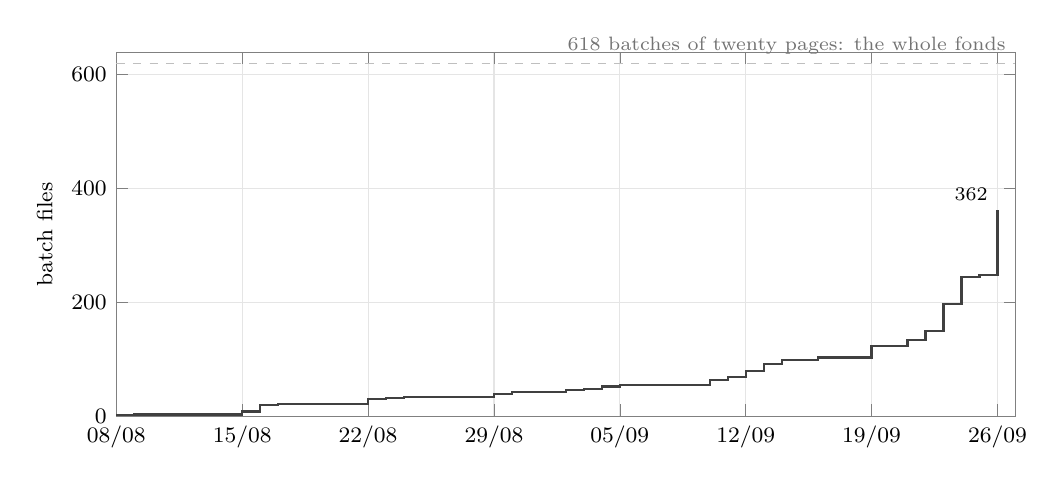
\begin{tikzpicture}
\begin{axis}[width=13cm,height=6.2cm,xmin=0,xmax=50,ymin=0,ymax=638,
  xtick={0,7,14,21,28,35,42,49},xticklabels={08/08,15/08,22/08,29/08,05/09,12/09,19/09,26/09},
  ylabel={batch files},grid=major,grid style={black!10},tick label style={font=\footnotesize},
  label style={font=\footnotesize},axis line style={black!50},clip=false]
\addplot[black!25,dashed,domain=0:50] {618};
\node[font=\scriptsize,text=black!55,anchor=south east] at (axis cs:50,618) {618 batches of twenty pages: the whole fonds};
\addplot[const plot,thick,black!75] coordinates {(0,2) (1,3) (2,3) (3,3) (4,3) (5,3) (6,3) (7,8) (8,20) (9,21) (10,21) (11,21) (12,21) (13,21) (14,30) (15,32) (16,33) (17,34) (18,34) (19,34) (20,34) (21,39) (22,43) (23,43) (24,43) (25,46) (26,48) (27,52) (28,54) (29,55) (30,55) (31,55) (32,55) (33,64) (34,68) (35,79) (36,92) (37,99) (38,99) (39,103) (40,103) (41,103) (42,123) (43,123) (44,133) (45,150) (46,197) (47,244) (48,247) (49,362)};
\node[font=\scriptsize,anchor=south east] at (axis cs:49,362) {362};
\end{axis}
\end{tikzpicture}
\caption{Batch files in the repository, day by day, from the first on 2026-08-08 to 2026-09-26: the date each \texttt{batch-NN.fr.tex} was first committed, cumulated. Each file is one pass of the model over at most twenty pages. The dashed line is the whole fonds at that rate. From the repository's git history, drawn on 2026-09-26 by \texttt{docs/study/figures.mjs}.}\label{fig:pace}
\end{figure}


Figure~\ref{fig:pace} gives the pace from the repository's history: the repository was opened on 7 August 2026, the first batch file was committed the next day and the 362nd on 26 September; 43 were committed in August and 319 in September, 115 of them on the last day, with up to eight passes running at once. At that rate the part of the fonds left to this edition is weeks of machine time. The human check is not. A batch of twenty pages of this hand, compared line by line with the facsimile by a mathematician who can read it, is an afternoon; the edition's 618 batches are some two and a half thousand hours of a rare kind of reader. That is the size of what is left, and it is the argument of this article in one number: the transcription is no longer the bottleneck and the checking is, and an edition that cannot say which of its pages a person has read is publishing a machine's confidence as though it were scholarship.

The protocol the edition proposes is the one its status file already encodes. A person opens a batch beside its facsimile, reads each transcribed line against the page, corrects the transcription at source with a note saying who checked it, and only then may declare the batch checked; the citation of every page in it then says so. Until then every citation names a machine pass and a date, and the address of the page does not move when the reading does.

\subsection{What the method permits, and what it does not}

The method permits a reading of a sixteen-thousand-page mathematical archive to be produced in months by one person's attention and a model's time, cited by folder, batch, page and pass, exported to TEI with its mathematics intact, placed beside an institution's own facsimile without copying it, and mined for registers of names, dates, letters and hands that each rest on a line. It does not produce a checked transcription; it does not encode the mathematics in a form a TEI processor can reason over; it does not yet validate against a customisation of its own; it does not decide who is a public figure with authority; and it does not remove the need for the person it was designed around.

\section{Conclusion}

This article has described a second edition built on the method of the first, and what a corpus of mathematics changes in it. The notation required a decision the ledgers did not: to carry mathematics as the TeX it was transcribed in, inside \texttt{<formula>}, rather than as a structure the transcription does not have, and to put the interpretation of that notation in a second register derived from the first. The size of the corpus turned the human check from a stated debt into the edition's main fact. And the rights turned the facsimile from a file the edition serves into one it points at, through a relay that holds nothing, so that the reading and its witness meet only on the reader's screen.

What remains is stated as three pieces of work. The first is an ODD for the TEI, declaring exactly what the converter emits and closing its value lists, validated on every build together with the renderer's refusals, so that a deposit is TEI and not XML and a refused file stops the build. The second is the division of \texttt{\textbackslash add} into the transcriber's supply and his insertion, by the rule of Section 9.2 and then by the facsimile. The third is the human check, which is the one on which every claim of the edition depends, and which is a question for the mathematicians who can read this hand, not for a model.

An edition is worth what its reader can check. For this fonds, checking means reading Grothendieck's hand against his page, which few people can do, over sixteen thousand pages, which nobody can do alone. What the method changes is that the reading exists, fully cited, before anyone checks it; what it cannot change is who must.

\section*{About the author}

Michel Hua is an independent consultant at Commutator, Paris, working with large organisations on data and cloud applications: platform migrations, data governance, and the adoption of generative AI. The editions he has built apply that discipline to archives institutions have digitised and few have read: the Hopper ledgers at the Whitney Museum, the Grothendieck fonds at Montpellier, and the mathematicians' manuscripts in Gallica. \texttt{michel@commutator.io}.

\section*{Declaration of Generative AI and AI-assisted technologies in the writing process}

During the preparation of this work the author used Claude Opus 5, Claude Opus 5.5, Claude Fable 5 and Claude Fable 5.1 (Anthropic), through Claude Code, in order to transcribe the pages of the fonds into the restricted transcription language described in Section 4, to write the modernised readings described in Section 5, to write the scripts, the converter, the relay, the interface and the derived registers described in Sections 6 and 7, to propose the findings described in Section 8, and to draft this article from the transcriptions and the derived data under the author's direction. After using these tools, the author reviewed and edited the content as needed and takes full responsibility for the content of the publication. The transcriptions have not been checked against the facsimiles by a person, and the article says so wherever a claim depends on them.

\section*{Data availability}

The transcriptions, the modernised readings, the TEI export, the scripts, the derived registers, the relay, the interface and the sources of this article are in the public repository at \url{https://github.com/Commutator-IO/grothendieck-project}; the interface is served at \url{https://grothendieck.commutator.io}. The software and the derived data are released under the repository's licence; this article under CC BY 4.0. The fonds is the University of Montpellier's and is under copyright; the transcriptions are unauthorised working documents, published for study and removed on request, and no image of the fonds is stored by the edition or reproduced in this article.

\section*{References}
\begin{list}{}{\setlength{\leftmargin}{1.5em}\setlength{\itemindent}{-1.5em}\setlength{\itemsep}{3pt}}
\item Colmez, Pierre, and Jean-Pierre Serre, eds. 2001. \emph{Correspondance Grothendieck--Serre}. Documents Mathématiques 2. Paris: Société Mathématique de France.
\item Crosilla, Giorgia, Lukas Klic, and Giovanni Colavizza. 2025. \qq{Benchmarking Large Language Models for Handwritten Text Recognition.} \emph{Journal of Documentation} 81 (7). Preprint: arXiv:2503.15195.
\item Cummings, James, and Pip Willcox. 2013. \qq{Stationers' Register Online: A Case Study of a Byte-Reduced TEI Schema for Digitization (tei\_corset).} \emph{Journal of the Text Encoding Initiative} 6. \url{https://doi.org/10.4000/jtei.926}.
\item Grothendieck Circle. n.d. \emph{Published Texts}. Edited by Leila Schneps. \url{https://webusers.imj-prg.fr/~leila.schneps/grothendieckcircle/pubtexts.php}.
\item Hua, Michel. 2026. \qq{A Machine Reads the Hopper Ledgers: Constrained Transcription, Mechanical TEI Export, and Checkability as the Editorial Condition.} Preprint, submitted to the Journal of the Text Encoding Initiative. \url{https://hopper.commutator.io/article/hopper-jtei.pdf}.
\item Humphries, Mark, Lianne C. Leddy, Quinn Downton, Meredith Legace, John McConnell, Isabella Murray, and Elizabeth Spence. 2025. \qq{Unlocking the Archives: Using Large Language Models to Transcribe Handwritten Historical Documents.} \emph{Historical Methods: A Journal of Quantitative and Interdisciplinary History} 58 (3). \url{https://doi.org/10.1080/01615440.2025.2500309}.
\item Maltsiniotis, Georges, ed. 2022. \emph{À la poursuite des champs}, by Alexandre Grothendieck. Documents Mathématiques 20. Paris: Société Mathématique de France.
\item Stokes, Peter A. 2015. \qq{Digital Approaches to Paleography and Book History: Some Challenges, Present and Future.} \emph{Frontiers in Digital Humanities} 2: 5. \url{https://doi.org/10.3389/fdigh.2015.00005}.
\item Strutz, Sabrina. 2026. \qq{A Multi-Dimensional Evaluation Framework for Assessing LLM Performance in TEI Encoding.} \emph{Journal of Open Humanities Data} 12 (1). \url{https://doi.org/10.5334/johd.484}.
\item TEI Consortium. 2026. \emph{TEI P5: Guidelines for Electronic Text Encoding and Interchange}. \url{https://tei-c.org/guidelines/p5/}.
\item Université de Montpellier. n.d. \emph{Archives Grothendieck}. \url{https://grothendieck.umontpellier.fr/}.
\item W3C. 2014. \emph{Mathematical Markup Language (MathML) Version 3.0}, 2nd ed. W3C Recommendation, 10 April 2014. \url{https://www.w3.org/TR/MathML3/}.
\end{list}

\appendix
\section{A complete transcribed page}

Page 8 of folder 19, batch 1, as the model wrote it in the restricted language, from the first pass of 22 August 2026 by Claude Opus 5; the TEI of Section 4.5 is derived from it. The page is \lf{19}{1}{on the site}, beside Montpellier's facsimile.

\begin{lstlisting}
\page{8}
qui s'expliciteront en termes des $\varphi_{ji} = f_{j} g_{i}$, et des
$\bar{\alpha}_{i}$, $\bar{\lambda}_{i}$ correspondants, ainsi
\[
  \left\{
  \begin{array}{l}
    \bar{\alpha}_{k} = \alpha_{k}(X_{k}) \circ \mathrm{pr}_{k} \\[2pt]
    \bar{\lambda}_{k,j,i} = \lambda_{kji}(X_{i}) \circ \mathrm{pr}_{i}
  \end{array}
  \right.
  \tag{3.9}
\]
\[
  \lambda_{kji} : \varphi_{ki} \longrightarrow \varphi_{kj} \circ \varphi_{ji}
  \tag{3.10}
\]

\begin{tikzcd}[column sep=small, row sep=small, nodes={font=\scriptsize}]
\varphi_{ki} \arrow[r, "\lambda_{kji}"] \arrow[d, no head] & \varphi_{kj}\varphi_{ji} \arrow[d, no head] \\
f_{k} g_{i} & f_{k}\, g_{j} f_{j}\, g_{i}
\end{tikzcd}

\note{la flèche provient du morphisme d'adjonction $\mathrm{id} \to g_{j} f_{j}$,
que l'auteur indique par une flèche verticale sous $g_{j} f_{j}$}

Les $(\varphi_{ji}, \lambda_{kji})$ sont reliées par des conditions exprimant
(1.5), (1.6), que nous n'expliciterons pas.

\marginal{pour $i = j = k$, $\lambda_{kji}$ n'est autre que $\lambda_{i}$}

[Le cas le plus intéressant est celui où les \struck{$\varphi$}
\add{$\alpha_{i}$} sont des isomorphismes (i.e. les $g_{i}$ pleinement
fidèles). Dans ce cas, \struck{\ill{}} on peut supposer
$\varphi_{i} = \mathrm{id}_{B_{i}}$,
$\alpha_{i} = \mathrm{id}_{\mathrm{id}_{B_{i}}}$, $\lambda_{i} = \mathrm{id}$.]

Les conditions (1.) \struck{les} dans les cas où deux des $i, j, k$ sont égaux,
avec $i = j$ ou $j = k$, \uncertain{ne montrent que} l'un des $\lambda_{kji}$
est l'identité, \ill{} de $\varphi_{kj} \varphi_{ji}$.
\note{ligne très surchargée ; le verbe reste douteux}

Il reste donc à examiner les cas (3.11) : a) \struck{$i$, $j$, $k$ deux à deux
différents} ; b) $i = k \neq j$, d'où
\[
  \mathrm{id}_{B_{i}} \longrightarrow \varphi_{ij} \circ \varphi_{ji}
  \qquad (i \neq j)
\]
\end{lstlisting}

\end{document}
